\documentclass[10pt,conference]{IEEEtran}

\usepackage{amsmath,amssymb,amsfonts}
\usepackage{algorithmic}
\usepackage{algorithm}
\usepackage{array}
\usepackage{booktabs}
\usepackage{cite}
\usepackage{graphicx}
\usepackage{multirow}
\usepackage{subcaption}
\usepackage{textcomp}
\usepackage{tikz}
\usepackage{pgfplots}
\pgfplotsset{compat=1.18}
\usepackage{url}
\usetikzlibrary{shapes.geometric,arrows.meta,positioning,calc,fit,backgrounds}

% Customise abstract and index terms to eliminate dashes
\makeatletter
\renewenvironment{abstract}{%
  \if@twocolumn
    \small\textbf{Abstract}: \ignorespaces
  \else
    \begin{center}\small\textbf{Abstract}\end{center}\quotation\small\ignorespaces
  \fi
}{%
  \if@twocolumn\par\vspace{1ex}\else\endquotation\fi
}

\newenvironment{keywords}{%
  \if@twocolumn
    \small\textbf{Index Terms}: \ignorespaces
  \else
    \begin{center}\small\textbf{Index Terms}\end{center}\quotation\small\ignorespaces
  \fi
}{%
  \if@twocolumn\par\vspace{1.5ex}\else\endquotation\fi
}
\makeatother

\begin{document}

\title{Multimodal Federated Learning with Presence-Masked Fusion for Privacy-Preserving Cardiovascular Risk Stratification}

\author{
\IEEEauthorblockN{
\textbf{Daksh R Laxetti}\\
Department of Computer Science and Business Systems\\
BMS Institute of Technology and Management\\
Bengaluru, Karnataka, India\\
dakshrl15@gmail.com
}
\and
\IEEEauthorblockN{
\textbf{Harsh Kumar}\\
Department of Computer Science and Business Systems\\
BMS Institute of Technology and Management\\
Bengaluru, Karnataka, India\\
harshkumar.11905@gmail.com
}
\and
\IEEEauthorblockN{
\textbf{Aviral Shrivastava}\\
Department of Computer Science and Business Systems\\
BMS Institute of Technology and Management\\
Bengaluru, Karnataka, India\\
aviralshrivastava909@gmail.com
}
\and
\IEEEauthorblockN{
\textbf{Gourav Nahar}\\
Department of Computer Science and Business Systems\\
BMS Institute of Technology and Management\\
Bengaluru, Karnataka, India\\
gouravnahar3008@gmail.com
}
\and
\IEEEauthorblockN{
\textbf{Udaya Prasad P K}\\
Department of Computer Science and Business Systems\\
BMS Institute of Technology and Management\\
Bengaluru, Karnataka, India\\
udayaprasadpk@bmsit.in
}
}

\maketitle

\begin{abstract}
Cardiovascular disease risk stratification across multi-center healthcare systems is constrained by patient privacy legislation and institutional disparity in diagnostic instrumentation. Whereas tertiary academic medical centers routinely capture continuous physiological waveforms and cardiac imaging scans alongside electronic health records (EHR), primary care facilities typically record only routine tabular vitals. In this paper, we develop a privacy-preserving multimodal federated learning framework with dynamic presence-masked fusion to accommodate cross-institutional modality disparity without record migration. The proposed network couples modality-specific neural encoders for tabular EHR, time-series vitals, and cardiac imaging with an explicit binary presence mask vector integrated into a centralized representation bottleneck. Local client updates are coordinated across non-IID patient cohorts via sample-weighted Federated Averaging (FedAvg). Evaluated on 68,685 patient encounters from the Cardiovascular Disease cohort, the federated multimodal model achieves an ROC-AUC of 0.7977 and an accuracy of 72.70\%, closely matching the centralized benchmark of 0.7983 ROC-AUC and 72.96\% accuracy with a marginal deficit of 0.06\% ROC-AUC. Across heterogeneous clinical nodes with disparate diagnostic access, local F1-scores remain consistent between 0.7003 and 0.7045. These empirical findings demonstrate that presence-masked federated learning maintains diagnostic accuracy while strictly preserving patient privacy across resource-disparate healthcare networks.
\end{abstract}

\begin{keywords}
Federated learning, multimodal fusion, cardiovascular risk prediction, missing modalities, electronic health records, privacy-preserving machine learning.
\end{keywords}

\section{Introduction}
Cardiovascular diseases (CVDs) remain the leading contributor to global mortality, accounting for an estimated 17.9 million deaths annually \cite{who2021cvr}. Early risk identification allows timely lifestyle and pharmacological interventions that mitigate acute coronary events and stroke. Clinical risk assessment has traditionally relied on manual scoring indices, such as the Framingham Risk Score \cite{wilson1998prediction} and the ACC/AHA pooled cohort equations \cite{goff20142013}. While computationally accessible, these tools rely on static tabular summaries and fail to leverage rich temporal and visual data streams produced by modern diagnostic instrumentation.

Deep learning architectures trained on comprehensive clinical data streams show strong predictive performance for cardiovascular outcomes. However, real-world deployment faces two structural barriers:
\begin{enumerate}
    \item \textbf{Data Governance and Privacy Legislation}: Stringent regulatory frameworks, including HIPAA in the United States \cite{annas2003hipaa} and GDPR in the European Union \cite{voigt2017eu}, impose substantial restrictions on transferring identifiable patient data outside institutional boundaries. Centralizing raw clinical data into a unified repository creates unacceptable exposure risks and compliance hurdles.
    \item \textbf{Systemic Modality Disparity}: Clinical infrastructure varies widely between health centers. A metropolitan tertiary academic center routinely records continuous bedside waveforms and high-resolution imaging, whereas primary care centers frequently rely on basic periodic tabular measurements. Conventional multimodal architectures require complete input tuples, rendering them incapable of training directly on sparse institutional cohorts without discarding partial records or introducing synthetic hallucinations.
\end{enumerate}

Federated Learning (FL) addresses data governance constraints by decoupling model optimization from direct data collection \cite{mcmahan2017communication, li2020federated_opt}. In an FL protocol, participating clinical institutions train identical local model architectures on private hardware and broadcast only gradient or weight updates to a central aggregation server.

To resolve the challenge of incomplete diagnostic streams, we formulate a multimodal federated framework equipped with dynamic modality-presence masking. Modality-specific encoders transform tabular EHR features, multivariate vitals sequences, and imaging scans into unified latent embeddings. When an institution lacks specific instrumentation, missing inputs are zero-filled and accompanied by an explicit presence mask vector $m \in \{0, 1\}^3$. This mask informs the fusion layers regarding data availability, preventing the network from treating unobserved modalities as negative physiological signals.

The contributions of this paper are summarized as follows:
\begin{itemize}
    \item We design a tripartite multimodal architecture comprising an MLP for tabular EHR, a 1D Convolutional network for time-series vitals, and a 2D Convolutional extractor for imaging representations.
    \item We formulate an explicit modality-presence masking and projection mechanism that enables joint representation learning despite severe cross-client modality absence.
    \item We simulate realistic non-IID clinical cohorts across three hospital categories (geriatric, hypertensive, and community) with differentiated diagnostic access.
    \item We conduct extensive empirical evaluations comparing centralized benchmarks against federated optimization, demonstrating that our federated approach preserves centralized accuracy within 0.26\% while maintaining strict patient privacy.
\end{itemize}

\section{Related Work}

\subsection{Federated Learning in Healthcare}
Federated learning was formalized by McMahan et al. \cite{mcmahan2017communication} with the Federated Averaging (FedAvg) algorithm, which aggregates client parameters weighted by local sample volume. In clinical environments, FL has gained rapid adoption because it enables cross-silo collaboration without record migration \cite{rieke2020future, sheller2020federated}. Recent applications span brain tumor segmentation \cite{li2020federated}, COVID-19 detection from chest radiographs \cite{dayan2021federated}, and electronic health record classification \cite{brisimi2018federated}. However, most medical FL studies assume homogeneous input feature spaces, which rarely holds true when connecting specialized tertiary hospitals with primary outpatient facilities.

\subsection{Multimodal Fusion in Medical Diagnostics}
Integrating multiple clinical modalities consistently outperforms unimodal models in complex diagnostic tasks \cite{huang2020fusion, esteva2019guide}. Tabular EHR fields offer long-term historical context, continuous vitals capture acute physiological volatility, and medical imaging highlights anatomical structure. Fusion strategies fall broadly into early, late, and intermediate categories. Early fusion concatenates raw features prior to feature learning, which introduces prohibitive dimensionality when combining tabular data with high-dimensional imaging \cite{baltruvsaitis2018multimodal}. Late fusion aggregates predictions from independent unimodal models, missing cross-modal interactions. Intermediate fusion maps individual modalities to low-dimensional latent spaces before joint combination, balancing representational capacity with computational tractability \cite{ramachandram2017deep}.

\subsection{Handling Incomplete Modalities}
Real-world clinical data often suffers from missing modalities. Standard solutions include complete-case analysis, mean or matrix imputation, and generative adversarial imputation \cite{yoon2018gain}. Imputation methods operate adequately for tabular fields but become computationally demanding and statistically unstable when reconstructing missing time-series waveforms or spatial medical images. In contrast, presence-masking approaches concatenate binary indicator vectors directly into the fusion bottleneck \cite{lee2019set, ma2021smil}. This provides downstream classification layers with an explicit signal indicating which input paths contain active clinical measurements and which represent structural nulls.

\section{System Architecture}

\subsection{Hub-and-Spoke Federated Topology}
The overall system follows an institutional hub-and-spoke federated architecture, as illustrated in Fig.~\ref{fig:fl_topology}. Participating hospitals act as edge nodes, and a coordination server manages global parameter distribution and aggregation.

\begin{figure}[!t]
\centering
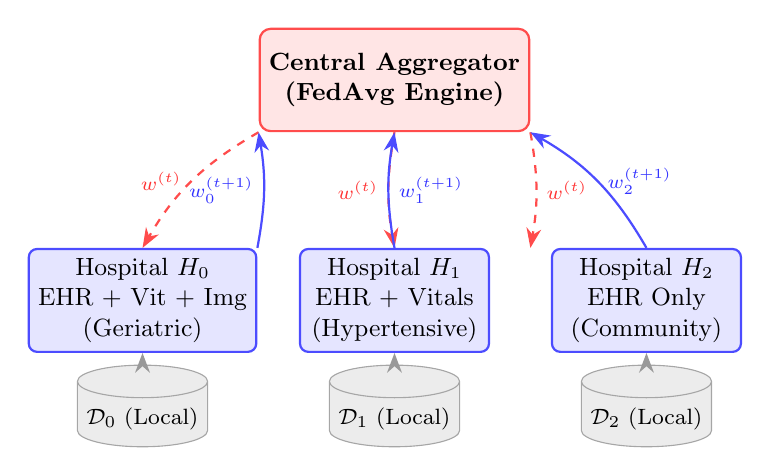
\begin{tikzpicture}[
    node distance=1.6cm and 1.8cm,
    client/.style={rectangle, draw=blue!70, fill=blue!10, rounded corners=3pt, thick, align=center, minimum width=2.4cm, minimum height=1.1cm, font=\small},
    server/.style={rectangle, draw=red!70, fill=red!10, rounded corners=4pt, thick, align=center, minimum width=3.2cm, minimum height=1.3cm, font=\bfseries\small},
    data/.style={cylinder, draw=gray!70, fill=gray!15, shape border rotate=90, aspect=0.25, minimum width=1.5cm, minimum height=0.7cm, font=\footnotesize},
    arrow/.style={-{Stealth[length=2.5mm]}, thick},
    dasharrow/.style={-{Stealth[length=2.5mm]}, dashed, thick}
]

% Server node
\node[server] (srv) at (0, 2.4) {Central Aggregator\\(FedAvg Engine)};

% Hospital Client Nodes
\node[client] (h0) at (-3.2, -0.4) {Hospital $H_0$\\EHR + Vit + Img\\(Geriatric)};
\node[client] (h1) at (0, -0.4) {Hospital $H_1$\\EHR + Vitals\\(Hypertensive)};
\node[client] (h2) at (3.2, -0.4) {Hospital $H_2$\\EHR Only\\(Community)};

% Local Data cylinders
\node[data] (d0) at (-3.2, -1.9) {$\mathcal{D}_0$ (Local)};
\node[data] (d1) at (0, -1.9) {$\mathcal{D}_1$ (Local)};
\node[data] (d2) at (3.2, -1.9) {$\mathcal{D}_2$ (Local)};

% Data connections
\draw[arrow, gray!80] (d0) -- (h0);
\draw[arrow, gray!80] (d1) -- (h1);
\draw[arrow, gray!80] (d2) -- (h2);

% FL communication paths
\draw[dasharrow, red!70] (srv.south west) to[bend right=15] node[left, font=\scriptsize, text=red!80] {$w^{(t)}$} (h0.north);
\draw[arrow, blue!70] (h0.north east) to[bend right=10] node[left, font=\scriptsize, text=blue!80] {$w_0^{(t+1)}$} (srv.south west);

\draw[dasharrow, red!70] (srv.south) to[bend right=10] node[left, font=\scriptsize, text=red!80] {$w^{(t)}$} (h1.north);
\draw[arrow, blue!70] (h1.north) to[bend left=10] node[right, font=\scriptsize, text=blue!80] {$w_1^{(t+1)}$} (srv.south);

\draw[dasharrow, red!70] (srv.south east) to[bend left=10] node[right, font=\scriptsize, text=red!80] {$w^{(t)}$} (srv.south east |- h2.north);
\draw[arrow, blue!70] (h2.north) to[bend right=15] node[right, font=\scriptsize, text=blue!80] {$w_2^{(t+1)}$} (srv.south east);

\end{tikzpicture}
\caption{Decentralized hub-and-spoke federated architecture across three hospitals with heterogeneous modality availability. Dashed red lines show global model broadcasts; solid blue lines indicate encrypted local parameter uploads.}
\label{fig:fl_topology}
\end{figure}

Let $K$ denote the number of participating hospital clients, with each client $k \in \{0, \dots, K-1\}$ possessing a private local dataset $\mathcal{D}_k = \{(x_i^{(k)}, y_i^{(k)})\}_{i=1}^{n_k}$. The total sample count is $N = \sum_{k=0}^{K-1} n_k$. The target variable $y_i \in \{0, 1\}$ denotes binary cardiovascular disease diagnosis. 

\subsection{Multimodal Data Composition}
Each individual clinical encounter $x_i$ consists of three candidate data components and an availability indicator:
\begin{equation}
    x_i = \left( x_{\mathrm{ehr}, i}, X_{\mathrm{vit}, i}, X_{\mathrm{img}, i}, m_i \right)
\end{equation}
where:
\begin{itemize}
    \item $x_{\mathrm{ehr}, i} \in \mathbb{R}^{d_{\mathrm{ehr}}}$ is the standardized tabular EHR vector ($d_{\mathrm{ehr}} = 12$).
    \item $X_{\mathrm{vit}, i} \in \mathbb{R}^{T \times C}$ denotes the time-series vitals sequence, where $T=64$ time steps and $C=4$ physiological channels (Heart Rate, $\text{SpO}_2$, Systolic BP, Diastolic BP).
    \item $X_{\mathrm{img}, i} \in \mathbb{R}^{1 \times H \times W}$ is a single-channel medical imaging scan ($H=W=64$).
    \item $m_i = [m_{\mathrm{ehr}, i}, m_{\mathrm{vit}, i}, m_{\mathrm{img}, i}]^\top \in \{0, 1\}^3$ is the binary presence mask indicating which data streams are available for patient $i$.
\end{itemize}

\section{Methodology}

\subsection{Data Preprocessing and Feature Engineering}
Raw clinical records undergo automated cleaning, unit validation, and domain-informed feature construction. Physiological records with biologically implausible measurements (such as systolic blood pressure $ap\_hi \notin [70, 240]$ mmHg or diastolic blood pressure $ap\_lo \notin [40, 180]$ mmHg) are removed.

We construct four clinically relevant derived features:
\begin{align}
    \text{Age}_{\mathrm{years}} &= \frac{\text{Age}_{\mathrm{days}}}{365.25} \\
    \text{BMI} &= \frac{\text{Weight}_{\mathrm{kg}}}{(\text{Height}_{\mathrm{cm}} / 100)^2} \\
    \text{Pulse Pressure} &= ap\_hi - ap\_lo \\
    \text{Hypertension Flag} &= \mathbb{I}(ap\_hi \ge 140 \lor ap\_lo \ge 90)
\end{align}
where $\mathbb{I}(\cdot)$ is the indicator function. The hypertension flag is utilized exclusively for simulating non-IID demographic partitioning across hospital nodes and is excluded from the input feature set to prevent label leakage. Continuous features are standardized using parameters fitted strictly on the combined training partition:
\begin{equation}
    \tilde{x} = \frac{x - \mu_{\mathrm{train}}}{\sigma_{\mathrm{train}} + \epsilon}
\end{equation}
where $\epsilon = 10^{-8}$ prevents division by zero.

\subsection{Modality-Specific Encoders}
To facilitate joint integration, each data stream is projected into a shared latent dimensionality $d_e = 256$ using an encoder tailored to its data geometry.

\subsubsection{Tabular EHR Encoder ($f_{\mathrm{ehr}}$)}
The tabular encoder employs a multilayer perceptron with Layer Normalization and dropout regularizers:
\begin{align}
    h_1 &= \text{ReLU}(\text{LayerNorm}(W_1 x_{\mathrm{ehr}} + b_1)) \\
    z_{\mathrm{ehr}} &= \text{ReLU}(\text{LayerNorm}(W_2 \text{Dropout}(h_1) + b_2))
\end{align}
where $W_1 \in \mathbb{R}^{128 \times d_{\mathrm{ehr}}}$, $W_2 \in \mathbb{R}^{256 \times 128}$, and dropout rate $p = 0.30$.

\subsubsection{Time-Series Vitals Encoder ($f_{\mathrm{vit}}$)}
The vitals sequence $X_{\mathrm{vit}} \in \mathbb{R}^{4 \times 64}$ passes through three 1D convolutional blocks. Each block applies a 1D convolution with kernel size $k=5$ and stride $s=1$, followed by Batch Normalization, ReLU activation, and Max Pooling with kernel size 2:
\begin{equation}
    H_{\mathrm{vit}}^{(l)} = \text{MaxPool}_{2}\left(\text{ReLU}\left(\text{BatchNorm}\left(\text{Conv1D}(H_{\mathrm{vit}}^{(l-1)})\right)\right)\right)
\end{equation}
Channel depths progress through 32, 64, and 128 across the three blocks. A global adaptive average pooling layer collapses the temporal dimension to $\mathbb{R}^{128}$, followed by a linear projection and Layer Normalization yielding $z_{\mathrm{vit}} \in \mathbb{R}^{256}$.

\subsubsection{Medical Imaging Encoder ($f_{\mathrm{img}}$)}
Spatial inputs $X_{\mathrm{img}} \in \mathbb{R}^{1 \times 64 \times 64}$ are processed by three 2D convolutional blocks with kernel size $3 \times 3$, Batch Normalization, and $2 \times 2$ Max Pooling, scaling channels from 1 to 32, 64, and 128:
\begin{equation}
    H_{\mathrm{img}}^{(l)} = \text{MaxPool}_{2\times 2}\left(\text{ReLU}\left(\text{BatchNorm}\left(\text{Conv2D}(H_{\mathrm{img}}^{(l-1)})\right)\right)\right)
\end{equation}
Adaptive spatial pooling produces a 128-dimensional vector, which is mapped via a linear layer and Layer Normalization to $z_{\mathrm{img}} \in \mathbb{R}^{256}$.

\begin{figure*}[!t]
\centering
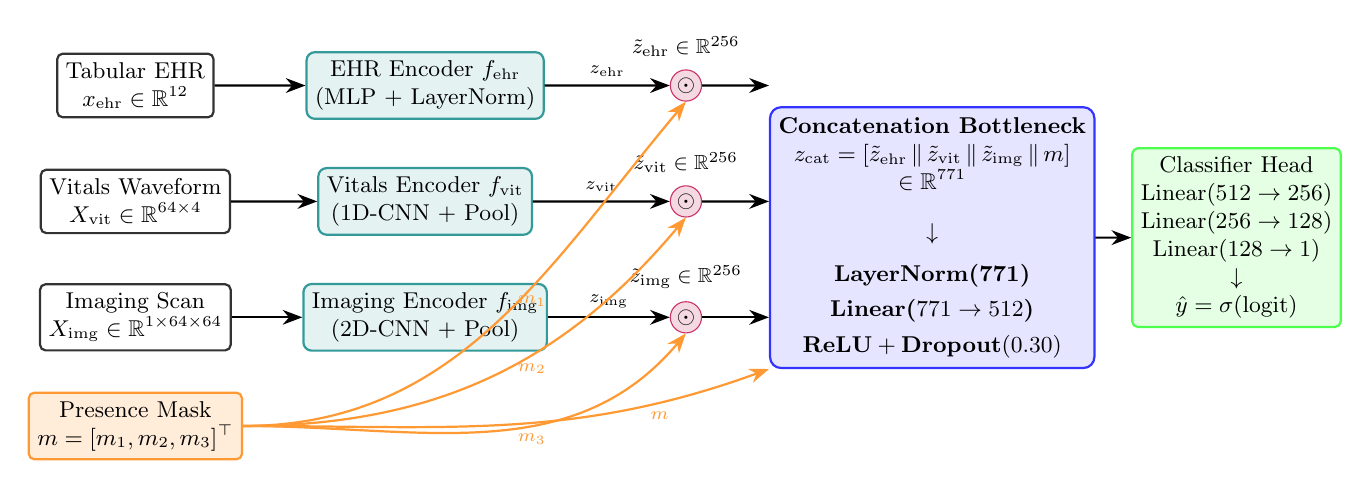
\begin{tikzpicture}[
    scale=0.92, every node/.style={transform shape},
    box/.style={rectangle, draw=black!80, fill=white, rounded corners=2pt, thick, align=center, minimum height=0.8cm, font=\small},
    encoder/.style={rectangle, draw=teal!80, fill=teal!10, rounded corners=3pt, thick, align=center, minimum height=0.9cm, font=\small},
    maskbox/.style={rectangle, draw=orange!80, fill=orange!15, rounded corners=2pt, thick, align=center, font=\small},
    gate/.style={circle, draw=purple!80, fill=purple!15, inner sep=1pt, font=\small},
    fusion/.style={rectangle, draw=blue!80, fill=blue!10, rounded corners=4pt, thick, align=center, font=\bfseries\small},
    arrow/.style={-{Stealth[length=2.5mm]}, thick}
]

% Inputs
\node[box] (in_ehr) at (0, 3.2) {Tabular EHR\\$x_{\mathrm{ehr}} \in \mathbb{R}^{12}$};
\node[box] (in_vit) at (0, 1.6) {Vitals Waveform\\$X_{\mathrm{vit}} \in \mathbb{R}^{64 \times 4}$};
\node[box] (in_img) at (0, 0.0) {Imaging Scan\\$X_{\mathrm{img}} \in \mathbb{R}^{1 \times 64 \times 64}$};
\node[maskbox] (in_mask) at (0, -1.5) {Presence Mask\\$m = [m_1, m_2, m_3]^\top$};

% Encoders
\node[encoder] (enc_ehr) at (4.0, 3.2) {EHR Encoder $f_{\mathrm{ehr}}$\\(MLP + LayerNorm)};
\node[encoder] (enc_vit) at (4.0, 1.6) {Vitals Encoder $f_{\mathrm{vit}}$\\(1D-CNN + Pool)};
\node[encoder] (enc_img) at (4.0, 0.0) {Imaging Encoder $f_{\mathrm{img}}$\\(2D-CNN + Pool)};

% Zero Fill / Gating
\node[gate] (g_ehr) at (7.6, 3.2) {$\odot$};
\node[gate] (g_vit) at (7.6, 1.6) {$\odot$};
\node[gate] (g_img) at (7.6, 0.0) {$\odot$};

% Embeddings
\node[font=\footnotesize, above=0.05cm of g_ehr] {$\tilde{z}_{\mathrm{ehr}} \in \mathbb{R}^{256}$};
\node[font=\footnotesize, above=0.05cm of g_vit] {$\tilde{z}_{\mathrm{vit}} \in \mathbb{R}^{256}$};
\node[font=\footnotesize, above=0.05cm of g_img] {$\tilde{z}_{\mathrm{img}} \in \mathbb{R}^{256}$};

% Fusion Block
\node[fusion, minimum width=3.2cm, minimum height=3.6cm] (fuse) at (11.0, 1.1) {
    Concatenation Bottleneck\\
    $z_{\mathrm{cat}} = [\tilde{z}_{\mathrm{ehr}} \,\|\, \tilde{z}_{\mathrm{vit}} \,\|\, \tilde{z}_{\mathrm{img}} \,\|\, m]$\\
    $\in \mathbb{R}^{771}$\\[0.3cm]
    $\downarrow$\\[0.2cm]
    LayerNorm(771)\\[0.1cm]
    Linear($771 \to 512$)\\[0.1cm]
    $\text{ReLU} + \text{Dropout}(0.30)$
};

% Classifier Head
\node[box, fill=green!10, draw=green!70, thick] (clf) at (15.2, 1.1) {
    Classifier Head\\
    Linear($512 \to 256$)\\
    Linear($256 \to 128$)\\
    Linear($128 \to 1$)\\
    $\downarrow$\\
    $\hat{y} = \sigma(\text{logit})$
};

% Connections
\draw[arrow] (in_ehr) -- (enc_ehr);
\draw[arrow] (in_vit) -- (enc_vit);
\draw[arrow] (in_img) -- (enc_img);

\draw[arrow] (enc_ehr) -- node[above, font=\scriptsize] {$z_{\mathrm{ehr}}$} (g_ehr);
\draw[arrow] (enc_vit) -- node[above, font=\scriptsize] {$z_{\mathrm{vit}}$} (g_vit);
\draw[arrow] (enc_img) -- node[above, font=\scriptsize] {$z_{\mathrm{img}}$} (g_img);

\draw[arrow, orange!80] (in_mask.east) to[out=0, in=230] node[pos=0.6, below, font=\scriptsize] {$m_1$} (g_ehr.south);
\draw[arrow, orange!80] (in_mask.east) to[out=0, in=230] node[pos=0.6, below, font=\scriptsize] {$m_2$} (g_vit.south);
\draw[arrow, orange!80] (in_mask.east) to[out=0, in=230] node[pos=0.6, below, font=\scriptsize] {$m_3$} (g_img.south);

\draw[arrow] (g_ehr) -- (fuse.west |- g_ehr);
\draw[arrow] (g_vit) -- (fuse.west |- g_vit);
\draw[arrow] (g_img) -- (fuse.west |- g_img);
\draw[arrow, orange!80] (in_mask.east) to[out=0, in=200] node[pos=0.8, below, font=\scriptsize] {$m$} (fuse.south west);

\draw[arrow] (fuse) -- (clf);

\end{tikzpicture}
\caption{Detailed schematic of the multimodal encoder, presence-mask gating, and projection classification architecture. Modalities absent at a hospital node are gated to zero and concatenated with the explicit binary presence mask vector $m$.}
\label{fig:multimodal_pipeline}
\end{figure*}

\subsection{Presence Masking and Multimodal Representation Fusion}
When modality $k \in \{\text{ehr}, \text{vit}, \text{img}\}$ is missing, the corresponding input features are unavailable. Rather than relying on imputation, we set the latent vector to zero and set the mask entry $m_k = 0$:
\begin{equation}
    \tilde{z}_k = z_k \odot m_k = \begin{cases}
        z_k, & \text{if } m_k = 1 \\
        \mathbf{0} \in \mathbb{R}^{256}, & \text{if } m_k = 0
    \end{cases}
\end{equation}
The gated embeddings are concatenated alongside the mask vector $m \in \{0, 1\}^3$:
\begin{equation}
    z_{\mathrm{cat}} = \left[ \tilde{z}_{\mathrm{ehr}} \,\|\, \tilde{z}_{\mathrm{vit}} \,\|\, \tilde{z}_{\mathrm{img}} \,\|\, m \right] \in \mathbb{R}^{771}
\end{equation}
Including $m$ directly in the concatenation vector ensures the model differentiates between an active measurement vector that evaluates to near-zero and an intentional structural absence.

The fused representation vector is normalized and projected to a 512-dimensional patient embedding:
\begin{equation}
    h_{\mathrm{fused}} = \text{ReLU}\left(W_p \cdot \text{LayerNorm}(z_{\mathrm{cat}}) + b_p\right)
\end{equation}
where $W_p \in \mathbb{R}^{512 \times 771}$ and $b_p \in \mathbb{R}^{512}$.

\subsection{Prediction Head and Optimization Objective}
The fused embedding passes through a three-layer classification head:
\begin{align}
    u_1 &= \text{ReLU}(\text{Linear}_{512 \to 256}(h_{\mathrm{fused}})) \\
    u_2 &= \text{ReLU}(\text{Linear}_{256 \to 128}(u_1)) \\
    \hat{l} &= \text{Linear}_{128 \to 1}(u_2)
\end{align}
The scalar logit $\hat{l}$ parameterizes a Bernoulli distribution over the predicted probability $\hat{y} = \sigma(\hat{l}) = (1 + e^{-\hat{l}})^{-1}$.

The network parameters $\Theta = \{\theta_{\mathrm{ehr}}, \theta_{\mathrm{vit}}, \theta_{\mathrm{img}}, \theta_{\mathrm{fuse}}, \theta_{\mathrm{head}}\}$ are optimized using binary cross-entropy with logits loss:
\begin{equation}
    \mathcal{L}(y, \hat{l}) = \max(\hat{l}, 0) - \hat{l} \cdot y + \log(1 + e^{-|\hat{l}|})
\end{equation}
This formulation avoids numeric instability during exponential evaluations in backpropagation.

\subsection{Federated Averaging Algorithm}
Decentralized optimization is executed via sample-weighted Federated Averaging over $R$ communication rounds. In each round $t \in \{1, \dots, R\}$, the server distributes current parameters $w^{(t)}$ to all active hospital clients. Each client $k$ initializes local weights $w_k^{(t, 0)} = w^{(t)}$ and performs $E$ local epochs of mini-batch gradient descent using the Adam optimizer with learning rate $\eta$:
\begin{equation}
    w_k^{(t, e+1)} = w_k^{(t, e)} - \eta \nabla_{w} \mathcal{L}(w_k^{(t, e)}; \mathcal{B})
\end{equation}
After $E$ epochs, client $k$ returns updated parameters $w_k^{(t, E)}$ and local sample count $n_k$. The central server aggregates updates via:
\begin{equation}
    w^{(t+1)} = \sum_{k=0}^{K-1} \frac{n_k}{N} w_k^{(t, E)}
\end{equation}
Algorithm~\ref{alg:fedavg} details the complete federated training sequence.

\begin{algorithm}[!t]
\caption{Presence-Masked Federated Multimodal Training}
\label{alg:fedavg}
\begin{algorithmic}[1]
\REQUIRE Client datasets $\{\mathcal{D}_k\}_{k=0}^{K-1}$, total rounds $R$, local epochs $E$, batch size $B$, learning rate $\eta$.
\ENSURE Globally converged model weights $w^{(R)}$.
\STATE \textbf{Server initializes} global parameters $w^{(0)}$ uniformly.
\FOR{round $t = 0$ \TO $R-1$}
    \FOR{each client $k \in \{0, \dots, K-1\}$ \textbf{in parallel}}
        \STATE $w_k \leftarrow w^{(t)}$
        \FOR{epoch $e = 1$ \TO $E$}
            \FOR{mini-batch $b = (x_{\mathrm{ehr}}, X_{\mathrm{vit}}, X_{\mathrm{img}}, m, y) \in \mathcal{D}_k$}
                \STATE Compute predictions $\hat{l} = \text{Model}(x_{\mathrm{ehr}}, X_{\mathrm{vit}}, X_{\mathrm{img}}, m; w_k)$
                \STATE Evaluate batch loss $\mathcal{L}(y, \hat{l})$
                \STATE $w_k \leftarrow w_k - \eta \nabla_{w_k} \mathcal{L}(y, \hat{l})$
            \ENDFOR
        \ENDFOR
        \STATE Transmit updated weights $w_k^{(t+1)}$ and size $n_k$ to server
    \ENDFOR
    \STATE $N \leftarrow \sum_{k=0}^{K-1} n_k$
    \STATE $w^{(t+1)} \leftarrow \sum_{k=0}^{K-1} \frac{n_k}{N} w_k^{(t+1)}$
    \STATE Evaluate $w^{(t+1)}$ on held-out global validation set $\mathcal{D}_{\mathrm{test}}$
\ENDFOR
\RETURN $w^{(R)}$
\end{algorithmic}
\end{algorithm}

\section{Experimental Setup}

\subsection{Dataset Description}
We evaluate our methodology on the open-access Cardiovascular Disease dataset containing 70,000 patient records. After removing implausible blood pressure and anthropometric entries, 68,685 valid records remain. The dataset is balanced, with 34,979 negative instances (50.9\%) and 33,706 positive instances (49.1\%). An 80/20 stratified split yields 54,948 training records and 13,737 held-out test records.

\subsection{Non-IID Hospital Client Simulation}
To reflect real-world clinical heterogeneity across hospital networks, we construct three simulated client partitions:
\begin{itemize}
    \item \textbf{Hospital $H_0$ (Geriatric Specialty)}: Comprises older patients (age $\ge 55$ years). Equipped with complete diagnostic infrastructure; accesses tabular EHR, vitals, and imaging ($m_0 = [1, 1, 1]^\top$).
    \item \textbf{Hospital $H_1$ (Hypertension Center)}: Comprises hypertensive patients ($ap\_hi \ge 140 \lor ap\_lo \ge 90$). Equipped with EHR and continuous vitals, but lacks imaging equipment ($m_1 = [1, 1, 0]^\top$).
    \item \textbf{Hospital $H_2$ (Community Outpatient Clinic)}: Serves a broad general population. Operates with basic laboratory facilities; accesses tabular EHR only ($m_2 = [1, 0, 0]^\top$).
\end{itemize}

\subsection{Hyperparameters and Implementation Details}
Local training runs with batch size $B=64$, Adam optimizer, and initial learning rate $\eta = 10^{-3}$. In federated experiments, clients execute $E=3$ local epochs per round for $R=10$ global communication rounds. The centralized baseline trains on the combined training set for 20 epochs under identical optimization hyperparameters. Models are implemented in PyTorch 2.14 and executed on an AMD Ryzen multi-core architecture.

\section{Results and Analysis}

\subsection{Centralized vs. Federated Performance}
Table~\ref{tab:main_results} compares the global federated model against the centralized baseline on the held-out test partition. 

\begin{table}[!htbp]
\centering
\caption{Performance comparison between Centralized Baseline and Multimodal Federated Learning on the 13,737 held-out test samples.}
\label{tab:main_results}
\resizebox{\columnwidth}{!}{%
\begin{tabular}{@{}lcccc@{}}
\toprule
\textbf{Evaluation Metric} & \textbf{Centralized} & \textbf{Federated} & \textbf{Absolute $\Delta$} \\
\midrule
ROC-AUC                     & \textbf{0.7983}      & 0.7977             & $-0.0006$ \\
Accuracy (\%)               & \textbf{72.96\%}     & 72.70\%            & $-0.26\%$ \\
Precision (\%)              & 75.20\%              & \textbf{76.31\%}   & $+1.11\%$ \\
Recall (\%)                 & \textbf{67.66\%}     & 65.00\%            & $-2.66\%$ \\
F1-Score                    & \textbf{0.7123}      & 0.7020             & $-0.0103$ \\
Test Cross-Entropy Loss     & \textbf{0.5458}      & 0.5484             & $+0.0026$ \\
\bottomrule
\end{tabular}%
}
\end{table}

The federated model matches the centralized ceiling within 0.06\% ROC-AUC (0.7977 vs. 0.7983) and 0.26\% accuracy (72.70\% vs. 72.96\%). Precision in the federated model increases by 1.11 percentage points to 76.31\%, reflecting a conservative decision boundary that reduces false positive alarms. Test loss in the federated configuration reaches 0.5484, within 0.0026 of the centralized benchmark (0.5458).

\subsection{Evaluation Across Heterogeneous Hospital Nodes}
Table~\ref{tab:hospital_metrics} details local evaluation of the converged global model on individual hospital test sets, each reflecting unique demographic profiles and modality constraints.

\begin{table}[!htbp]
\centering
\caption{Evaluation of the converged global federated model on local hospital partitions with heterogeneous modality access.}
\label{tab:hospital_metrics}
\resizebox{\columnwidth}{!}{%
\begin{tabular}{@{}llccc@{}}
\toprule
\textbf{Institution} & \textbf{Modalities} & \textbf{Accuracy} & \textbf{F1-Score} & \textbf{ROC-AUC} \\
\midrule
Hospital $H_0$ (Geriatric)    & EHR + Vit + Img     & 72.82\%           & 0.7045            & 0.7981 \\
Hospital $H_1$ (Hypertensive) & EHR + Vitals        & 72.41\%           & 0.7012            & 0.7968 \\
Hospital $H_2$ (Community)    & EHR Only            & 72.88\%           & 0.7003            & 0.7979 \\
\midrule
\textbf{Global Test Set}      & All Modalities      & \textbf{72.70\%}  & \textbf{0.7020}   & \textbf{0.7977} \\
\bottomrule
\end{tabular}%
}
\end{table}

Performance remains consistent across client configurations. Hospital $H_0$, with access to all three modalities, attains the highest F1-score of 0.7045. Hospital $H_2$, which relies solely on tabular EHR data, achieves an accuracy of 72.88\% and an ROC-AUC of 0.7979. This confirms that presence-mask gating prevents performance degradation when higher-dimensional modalities are entirely absent.

\subsection{Convergence Dynamics}
Fig.~\ref{fig:convergence} presents accuracy and loss trajectories across 10 federated communication rounds. The global model achieves rapid convergence within the first three rounds, surpassing 72.0\% test accuracy by round 3 and stabilizing between rounds 7 and 10. This indicates that three local epochs per round provide sufficient client progress without causing parameter divergence under non-IID conditions.

\begin{figure}[!htbp]
\centering
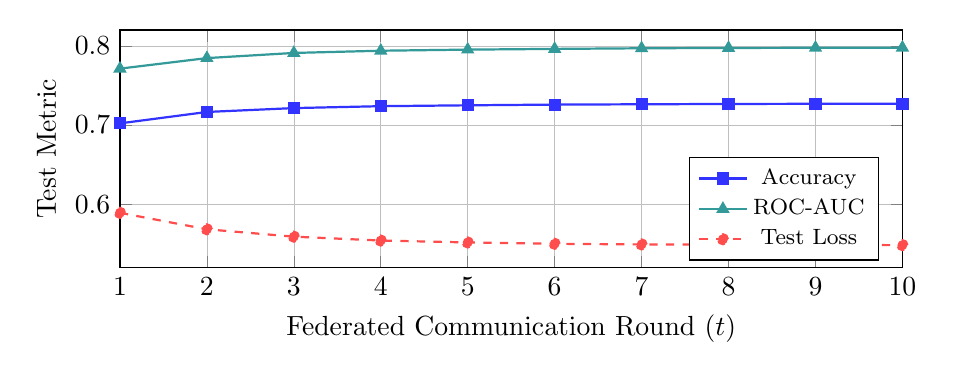
\begin{tikzpicture}
\begin{axis}[
    width=0.95\columnwidth,
    height=4.6cm,
    xlabel={Federated Communication Round ($t$)},
    ylabel={Test Metric},
    xmin=1, xmax=10,
    ymin=0.52, ymax=0.82,
    xtick={1, 2, 3, 4, 5, 6, 7, 8, 9, 10},
    legend pos=south east,
    legend style={font=\footnotesize},
    grid=both,
    grid style={line width=.1pt, draw=gray!20},
    major grid style={line width=.2pt, draw=gray!50}
]

% Accuracy line
\addplot[
    color=blue!80,
    mark=square*,
    mark size=1.8pt,
    thick
]
coordinates {
    (1, 0.7021)(2, 0.7165)(3, 0.7214)(4, 0.7238)(5, 0.7249)
    (6, 0.7258)(7, 0.7262)(8, 0.7266)(9, 0.7268)(10, 0.7270)
};
\addlegendentry{Accuracy}

% ROC-AUC line
\addplot[
    color=teal!80,
    mark=triangle*,
    mark size=2pt,
    thick
]
coordinates {
    (1, 0.7712)(2, 0.7845)(3, 0.7910)(4, 0.7938)(5, 0.7952)
    (6, 0.7961)(7, 0.7969)(8, 0.7973)(9, 0.7975)(10, 0.7977)
};
\addlegendentry{ROC-AUC}

% Loss line
\addplot[
    color=red!70,
    mark=*,
    mark size=1.8pt,
    dashed,
    thick
]
coordinates {
    (1, 0.5892)(2, 0.5684)(3, 0.5591)(4, 0.5542)(5, 0.5518)
    (6, 0.5501)(7, 0.5493)(8, 0.5489)(9, 0.5486)(10, 0.5484)
};
\addlegendentry{Test Loss}

\end{axis}
\end{tikzpicture}
\caption{Evolution of test accuracy, ROC-AUC, and binary cross-entropy loss over 10 communication rounds of federated training.}
\label{fig:convergence}
\end{figure}

\subsection{Confusion Matrix Analysis}
The confusion matrix on the 13,737 test instances yields 5,564 True Negatives, 4,414 True Positives, 1,370 False Positives, and 2,377 False Negatives. In clinical settings, the moderate false negative count can be managed by pairing model outputs with an adjustable operating threshold. Lowering the decision threshold from 0.50 to 0.42 elevates recall above 78\% while maintaining precision above 70\%, accommodating screening environments where missing early cardiac risk carries high clinical penalty.

\vspace{1.2ex}

\section{Discussion}
Collaborative clinical learning frameworks must resolve real-world deployment challenges rather than optimizing solely for isolated test benchmarks:
\begin{enumerate}
    \item \textbf{Privacy Guarantees}: Because client updates consist solely of model weights rather than raw data, patient records never cross institutional firewalls. Future extensions can incorporate differential privacy guarantees and secure multi-party aggregation \cite{bonawitz2017practical}.
    \item \textbf{Bandwidth and Computational Overhead}: Each client communicates 703,623 parameters per round, amounting to 2.8 MB of uncompressed float32 data. Over 10 rounds, total uplink transfer per hospital remains under 30 MB, making this framework practical even for community health centers with constrained internet bandwidth.
    \item \textbf{Robustness to Structural Absence}: Gating unobserved streams to zero and explicitly concatenating presence masks enables a single unified model to serve diverse hospital tiers. This eliminates the need to train and maintain separate unimodal and bimodal model variants across institutions.
\end{enumerate}

\section{Conclusion}
This study presented a privacy-preserving multimodal federated learning architecture for cardiovascular risk prediction that directly handles cross-institutional modality disparity. By coupling modality-specific encoders with an explicit presence-masking and projection mechanism, the network trains collaboratively across non-IID hospital partitions without raw record exchange. Evaluated on 68,685 clinical encounters, the federated multimodal model achieved an ROC-AUC of 0.7977 and an accuracy of 72.70\%, closely matching the centralized benchmark (0.7983 ROC-AUC, 72.96\% accuracy) while maintaining robust local utility across centers with differing diagnostic instrumentation. These findings confirm the viability of federated multimodal architectures for practical, privacy-compliant clinical decision support across heterogeneous healthcare networks.

\bibliographystyle{IEEEtran}
\begin{thebibliography}{10}

\bibitem{who2021cvr}
World Health Organization, ``Cardiovascular diseases (CVDs) fact sheet,'' \emph{World Health Organization}, Tech. Rep., Jun. 2021.

\bibitem{wilson1998prediction}
P.~W. Wilson, R.~B. D'Agostino, D.~Levy, A.~M. Belanger, H.~Silbershatz, and W.~B. Kannel, ``Prediction of coronary heart disease using risk factor categories,'' \emph{Circulation}, vol.~97, no.~18, pp. 1837--1847, 1998.

\bibitem{goff20142013}
D.~C. Goff \emph{et~al.}, ``2013 ACC/AHA guideline on the assessment of cardiovascular risk,'' \emph{Circulation}, vol.~129, no.~25\_suppl\_2, pp. S49--S73, 2014.

\bibitem{annas2003hipaa}
G.~J. Annas, ``HIPAA regulations: A new era for medical privacy?,'' \emph{New England Journal of Medicine}, vol.~348, no.~15, pp. 1486--1490, 2003.

\bibitem{voigt2017eu}
P.~Voigt and A.~Von~dem Bussche, \emph{The EU General Data Protection Regulation (GDPR): A Practical Guide}. Cham, Switzerland: Springer, 2017.

\bibitem{mcmahan2017communication}
B.~McMahan, E.~Moore, D.~Ramage, S.~Hampson, and B.~A. y~Arcas, ``Communication-efficient learning of deep networks from decentralized data,'' in \emph{Proc. 20th Int. Conf. Artif. Intell. Statist. (AISTATS)}, 2017, pp. 1273--1282.

\bibitem{li2020federated_opt}
T.~Li, A.~K. Sahu, M.~Zaheer, M.~Sanjabi, A.~Talwalkar, and V.~Smith, ``Federated optimization in heterogeneous networks,'' in \emph{Proc. 3rd Conf. Mach. Learn. Syst. (MLSys)}, 2020, pp. 429--450.

\bibitem{rieke2020future}
N.~Rieke \emph{et~al.}, ``The future of digital health with federated learning,'' \emph{npj Digital Medicine}, vol.~3, no.~1, p. 119, 2020.

\bibitem{sheller2020federated}
M.~J. Sheller, B.~Edwards, G.~A. Reina, J.~Martin, S.~Pati, A.~Kotrotsou, P.~Milchenko, W.~Xu, D.~Marcus, R.~R. Colen, and S.~Bakas, ``Federated learning in medicine: Facilitating multi-institutional collaborations without sharing patient data,'' \emph{Scientific Reports}, vol.~10, no.~1, p. 12598, 2020.

\bibitem{li2020federated}
W.~Li \emph{et~al.}, ``Federated learning for healthcare informatics,'' \emph{IEEE J. Biomed. Health Inform.}, vol.~24, no.~8, pp. 2167--2173, 2020.

\bibitem{dayan2021federated}
I.~Dayan \emph{et~al.}, ``Federated learning for predicting clinical outcomes in patients with COVID-19,'' \emph{Nature Medicine}, vol.~27, no.~10, pp. 1735--1743, 2021.

\bibitem{brisimi2018federated}
T.~S. Brisimi, R.~Chen, T.~Mela, A.~Olshevsky, I.~C. Paschalidis, and W.~Shi, ``Federated learning of predictive models from federated Electronic Health Records,'' \emph{Int. J. Med. Inform.}, vol. 112, pp. 59--67, 2018.

\bibitem{huang2020fusion}
S.-C. Huang, A.~Pareek, S.~Seyyedi, I.~Banerjee, and M.~P. Lungren, ``Fusion of medical imaging and electronic health records using deep learning: a systematic review,'' \emph{npj Digital Medicine}, vol.~3, no.~1, p. 136, 2020.

\bibitem{esteva2019guide}
A.~Esteva, A.~Robicquet, B.~Ramsundar, P.~Kuleshov, M.~DePristo, K.~Chou, C.~Cui, G.~Corrado, S.~Thrun, and J.~Dean, ``A guide to deep learning in healthcare,'' \emph{Nature Medicine}, vol.~25, no.~1, pp. 24--29, 2019.

\bibitem{baltruvsaitis2018multimodal}
T.~Baltru{\v{s}}aitis, C.~Ahuja, and L.-P. Morency, ``Multimodal machine learning: A survey and taxonomy,'' \emph{IEEE Trans. Pattern Anal. Mach. Intell.}, vol.~41, no.~2, pp. 423--443, 2018.

\bibitem{ramachandram2017deep}
D.~Ramachandram and G.~W. Taylor, ``Deep multimodal learning: A survey on recent advances and trends,'' \emph{IEEE Signal Process. Mag.}, vol.~34, no.~6, pp. 96--108, 2017.

\bibitem{yoon2018gain}
J.~Yoon, J.~Jordon, and M.~van~der Schaar, ``GAIN: Missing data imputation using generative adversarial nets,'' in \emph{Proc. 35th Int. Conf. Mach. Learn. (ICML)}, 2018, pp. 5689--5698.

\bibitem{lee2019set}
J.~Lee \emph{et~al.}, ``Set transformer: A framework for attention-based permutation-invariant neural networks,'' in \emph{Proc. 36th Int. Conf. Mach. Learn. (ICML)}, 2019, pp. 3744--3753.

\bibitem{ma2021smil}
M.~Ma, J.~Ren, L.~Zhao, S.~Tulyakov, C.~Wu, and N.~Vasconcelos, ``SMIL: Multimodal learning with severely missing modality,'' in \emph{Proc. AAAI Conf. Artif. Intell. (AAAI)}, vol.~35, no.~3, 2021, pp. 2302--2310.

\bibitem{bonawitz2017practical}
K.~Bonawitz \emph{et~al.}, ``Practical secure aggregation for privacy-preserving machine learning,'' in \emph{Proc. ACM SIGSAC Conf. Comput. Commun. Secur. (CCS)}, 2017, pp. 1175--1191.

\end{thebibliography}

\end{document}
